\section{Dommage de casques}
\vspace{.2cm}

\noindent
Un échantillon aléatoire de 50~casques de motos et de courses automobiles a été testé à l’impact. Des
dommages ont été observés pour 18 d’entre eux. 

%%%%%
\begin{itemize}[label={},itemindent=-2em,leftmargin=2em]
    \item \textbf{Question~5~:} Construire un intervalle de confiance à $95\%$ pour la vraie proportion des casques qui
    montreraient des dommages à ce test.
\end{itemize}
\vspace{.2cm}

\noindent
Pour répondre à cette question nous avons utilisé la formule~\ref*{eq:ic_grand2}, pour le code python on a utiliser la fonction 
\textit{intervalle\_confiance(n, x, ic)} réalisé à la question~3.

\vspace{.2cm}


\begin{lstlisting}[style=myPython, caption=Code Python question 5, frame=lines]
n_casques = 50
n_dommages = 18
borne_inf_dommages_95, borne_supp_dommages_95 = intervalle_confiance(n_casques, n_dommages, 95)

print("Casques endommagés")
print("\t --> Borne inférieur à 95%:", borne_inf_dommages_95)
print("\t --> Borne supérieur à 95%:", borne_supp_dommages_95, end="\n\n")
\end{lstlisting}

\begin{lstlisting}[style=myLog, caption=Résultat du code, frame=lines]
Casques endommagés
    --> Borne inférieur à 95%: 0.227
    --> Borne supérieur à 95%: 0.493
\end{lstlisting}



\vspace{.5cm}


%%%%%
\begin{itemize}[label={},itemindent=-2em,leftmargin=2em]
    \item \textbf{Question~6~:} En utilisant un estimateur ponctuel de p à partir de 50~casques, combien de casques
    doivent être testés pour avoir une erreur inférieure à 0,02 pour l’IC à $95\%$ de la proportion p~?
\end{itemize}
\vspace{.2cm}

\noindent
Pour répondre à cette question, nous avons utilisé la formule \ref*{eq:n} \textit{(cf. Question~4)}.

\vspace{.2cm}


\begin{lstlisting}[style=myPython, caption=Code Python question 6, frame=lines]
ic = 95
alpha = 1 - ic / 100
p = 18/50
err = .02
z = stats.norm.ppf(1 - (alpha / 2), loc=0, scale=1)
n = (z/err)**2 * p*(1-p)
n = np.ceil(n)

print("Nombre de casque à tester:", n, end='\n\n')
\end{lstlisting}

\begin{lstlisting}[style=myLog, caption=Résultat du code, frame=lines]
Nombre de casque à tester: 2213.0
\end{lstlisting}

\vspace{.5cm}


%%%%%
\begin{itemize}[label={},itemindent=-2em,leftmargin=2em]
    \item \textbf{Question~7~:} Quelle doit être la taille de l’échantillon pour obtenir une erreur inférieure à 0,02 pour
    l’IC à $95\%$ de la proportion $p$. Vous considérerez que vous ne connaissez ni la valeur de $p$ ni celle
    de $\hat{p}$~? Vous déterminerez la valeur $p$ pour que la fonction $n=f(p)$ soit maximale.
\end{itemize}

\begin{figure}[!h]
    \centering
    \begin{minipage}{.48\linewidth}
        En théorie le cas le plus défavorable a lieu quand $p=0.5$ (soit $n$ maximale), mais pour répondre à la question et vérifier cette théorie nous avons décidé de créer un vecteur $p$, contenant des valeurs de 0 à 1 par pas de 0,1. En calculant $n$ avec les différentes valeurs de $p$, nous pouvons obtenir 
        la valeur max de $n$ avec la fonction \textit{max}. \\

        Pour illustrer et vérifier la valeur obtenue, on a tracé la fonction $n=f(p)$ et la valeur max obtenue, on trouve bien une valeur de $p=0.5$ \textit{(cf. Figure~\ref*{fig:figure1})}.
    \end{minipage}\hfill
    \begin{minipage}{.48\linewidth}
        \begin{center}
            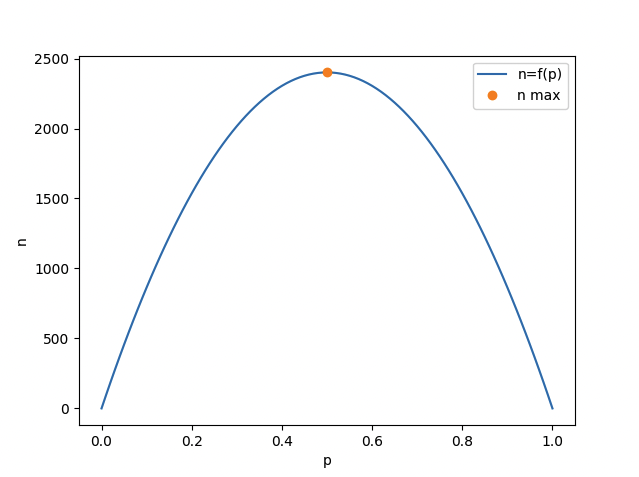
\includegraphics[width=1\textwidth]{img/figure1.png}
            \caption{\label{fig:figure1}Courbe de $n=f(p)$}
        \end{center}
    \end{minipage}
\end{figure}

\noindent
Nous avons utilisé la formule \ref*{eq:n} \textit{(cf. Question~4)}.

\vspace{.2cm}


\begin{lstlisting}[style=myPython, caption=Code Python question 7, frame=lines]
ic = 95
alpha = 1 - ic / 100
err = .02
z = stats.norm.ppf(1 - (alpha / 2), loc=0, scale=1)
p = np.linspace(0, 1, 101)
n = (z/err)**2 * p*(1-p)
index_n_max = np.where(n == max(n))
n = np.ceil(float(n[index_n_max]))

print("Question 7:\n", "Nombre de casque à tester:", n, end='\n\n')
\end{lstlisting}

\begin{lstlisting}[style=myLog, caption=Résultat du code, frame=lines]
Nombre de casque à tester: 2401.0
\end{lstlisting}

